% Reflexion der eigenen Arbeit, ungelöste Probleme, weitere Ideen.

\chapter{Ausblick}\label{ausblick}
In diesem Kapitel werden möglich nächste Schritte für die Weiterentwicklung des DlmsQuickAccess aufgelistet.
Diese basieren auf  Rückmeldungen von Nutzern, Erkenntnissen aus dem Entwicklungsprozess oder auf geplanten Features, welche in den sechs Sprints nicht umgesetzt werden konnten.  
Diese Arbeiten wurden in \ac{ADO} als User Story oder Bug erfasst, so dass sie von der Landis+Gyr priorisiert und eingeplant werden können.
Ein Ausschnitt aus diesem Backlog ist in Abbildung \ref{fig:ADOBacklog} gezeigt.
Ebenfalls reflektiert der Autor der Arbeit das Projekt.
\begin{figure}[H]
   \centering
   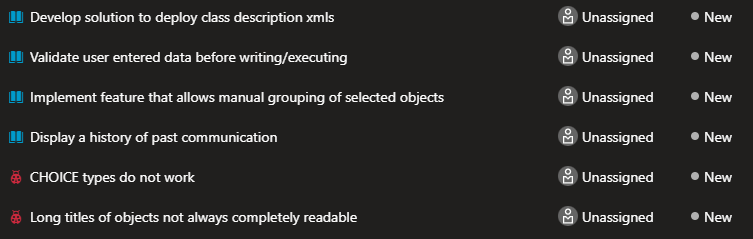
\includegraphics[width=1.0\textwidth]{gfx/ADOBacklog.png}
   \caption{
      Ausschnitt aus dem Backlog in \ac{ADO}
      }
   \label{fig:ADOBacklog}
\end{figure}


\section{Nächste Schritte}\label{nextSteps}
In den folgenden Abschnitten werden mögliche nächste Schritte aufgelistet.
Die Reihenfolge entspricht nicht einer Priorisierung sondern ist zufällig.

\subsection{Class Descriptions}
Die Class Descriptions, welche verwendet werden, um zusätzliche Informationen zu dem \ac{COSEM}-Objekten des Object Models darzustellen, sind Teil der Anwendung und werden bei der Installation auf den Rechner des Nutzers kopiert.
Um Änderungen an den Class Descriptions an die Nutzer zu verteilen, muss jeweils eine neue Version der Anwendung veröffentlicht werden.
Da dies während dieses Projektes regelmässig gemacht wurde, waren die Class Descriptions bisher immer aktuell.
In der Zukunft sollte jedoch eine Lösung gefunden werden, bei welcher die Class Descriptions unabhängig von der Anwendung aktualisiert werden können.

\subsection{Eingabevalidierung}
Dank den Class Descriptions verfügt der DlmsQuickAccess über detaillierte Angaben zu den Typen der Attribute.
Diese sollen verwendet werden, um die Eingaben der Nutzer zu validieren, bevor diesen an den Zähler geschickt werden.
So soll der Nutzer beispielsweise darauf hingewiesen werden, wenn er bei einem Integer Attribut unerlaubte Eingaben wie Text oder eine Fliesskommazahl macht.

\subsection{Optimierung für unterschiedliche Fenstergrössen}
In der Evaluation der Usability wurde (\ref{evalUsabilty}) festgehalten, dess Teile der Anwendung fehlerhaft dargestellt werden, wenn die Fenstergrösse der Anwendung von der Norm abweicht.
Die Anwendung soll so optimiert werden, dass auch bei kleineren Fenster alle Informationen leserlich sind.
Unterschiedliche Fenstergrössen und Seitenverhältnisse sollen getestet werden und nötige Anpassungen an der Anwendung gemacht werden.

\subsection{File Picker}\label{ausblick:filePicker}
Wird die Anwendung beim ersten Start ohne Konfigurationsdatei ausgeführt, so ist es für den Nutzer nicht möglich den DlmsQuickAccess richtig verwenden zu können.
Das Fenster, welches in Abbildung \ref{fig:welcomeScreenEmpty} gezeigt ist, weist ihn darauf hin, dass er die Anwendung über Eine *.dlmsquickaccess starten soll.
Es sollte jedoch auch möglich sein, eine Konfigurationsdatei mittels File Picker auswählen zu können.
In Abschnitt \ref{s3configvorgehen} ist beschrieben, wieso dies noch nicht umgesetzt werden konnte.

\begin{figure}[H]
   \centering
   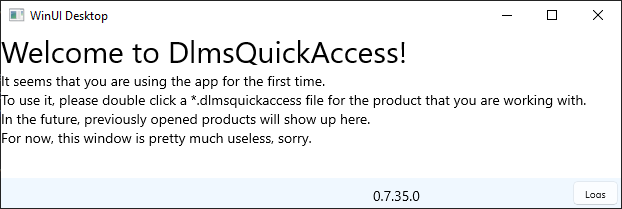
\includegraphics[width=1.0\textwidth]{gfx/welcomeScreenEmpty.png}
   \caption{
       Fenster des DlmsQuickAccess, welches erscheint, wenn die Anwendung ohne Konfiguration gestartet wird.
   }
   \label{fig:welcomeScreenEmpty}
\end{figure}

\subsection{Continuous Deployment}
Das Ziel von Continuous Deployment ist es, dass Änderungen am Code, welche alle Validierungsschritte (z.B. Tests) erfolgreich durchlaufen konnten, automatisch an Nutzer ausgeliefert werden \parencite{atlassian_2019}.
Im Text zum ersten Sprint (\ref{s1}) wurde erklärt, dass die Anwendung bei jedem Commit gebaut und wie das Deployment an die Nutzer funktioniert.
Werden diese beiden Aspekte kombiniert, so spricht man von Continuous Deployment.
Dies war bisher noch nicht möglich, weil \ac{ADO} keinen Zugriff auf das Netzwerkverzeichnis hat, auf welchem die Artefakte der Anwendung abgelegt sind.
Wird in Zukunft ein Continuous Deployment eingerichtet, so bringt dies den Vorteil, dass die Entwickler sich nicht selbst um die Veröffentlichung der Anwendung kümmern müssen und dabei auch keine Fehler machen können.

\subsection{DMT2 Quick Access ablösen}\label{moreUser}
Wie im Abschnitt \ref{survey} beschrieben, wurden für diese Arbeit bewusst nur Entwickler aus Cham in den Entwicklungsprozess miteinbezogen.
Diese verwenden den DlmsQuickAccess in Kombination mit den Referenzprodukten der Picasso Platform.
Um die alte Software vollständig abzulösen, müssen Konfigurationen für weitere Produkte bereitgestellt sowie alle Entwickler mit dem DlmsQuickAccess bekannt gemacht werden.


\subsection{Sourcecode Organisieren}\label{ausblick:ats_split}
In diesem Projekt wurden Code von anderen C\# Anwendungen der Landis+Gyr verwendet.
Dazu wurden die Repositories dieser Anwendungen in das Repository des DlmsQuickAccess kopiert.
Wie das umgesetzt wurde, ist im Abschnitt \ref{atsUmsetztung} aufgeführt. 
Ein möglicher nächster Schritt wäre es, diese Abhängigkeiten neu zu organisieren.
Dazu müssten jene Teile des Codes, welche von DlmsQuickAccess benötigt werden, als NuGet Paket bereitgestellt werden.


\subsection{Testagent mit Zähler}
Im Abschnitt \ref{Integrationstests} wurde beschrieben, dass für das Ausführen der Integrationstests ein angeschlossener Stromzähler benötigt wird.
Beim Testagent, welcher die Tests in \ac{ADO} ausführt, ist kein solcher Zähler vorhanden.
Deshalb konnten die Integrationstest nur lokal ausgeführt werden.
Um in Zukunft sicherstellen zu können, dass neue Änderungen keine bestehenden Funktionen zerstören, wäre es ein möglicher nächster Schritt, einen Testagent mit angeschlossenem Stromzähler aufzusetzen.

\subsection{SonarQube}
In Abschnitt \ref{s6:sonar} wurde erklärt, wieso im Rahmen dieser Arbeit lediglich eine lokale Instanz des Qualitätssicherungstools SonarQube eingesetzt wurde.
Für den Unterhalt und die Weiterentwicklung der Anwendung sollte jedoch eine Instanz auf einem Server eingesetzt werden, welche mit dem \ac{CI} Server verbunden ist.
Dies hätte zwei Vorteile:
\begin{itemize}
   \item Die Berichte zu Codequalität werden bei jeder Änderung des Codes automatisch erstellt. 
Entwickler müssen sich nicht selber darum kümmern.
   \item Die Metriken zur Qualität der Anwendung sind für alle Personen einsehbar.
\end{itemize}


\subsection{Zertifikat für die Signierung der Anwendung}\label{ausblick:cert}
Im Abschnitt \ref{deployment} wurde erklärt, wie das Deployment der Anwendung umgesetzt wurde.
Dabei wurde die Schwierigkeit beschrieben, dass jeder Nutzer der Anwendung manuell ein Zertifikat einrichten muss, um die Anwendung installieren zu können.
Dieses Zertifikat gibt den Autor dieser Arbeit und nicht die Landis+Gyr als Ersteller der Anwendung an.
Das Zertifikat könnte durch eines der Landis+Gyr ersetzt werden, welches auf den Rechnern der Nutzer bereits vorhanden ist.


\subsection{History}
Vergangene Kommunikationen und deren Resultate sollen gespeichert und für die Nutzer dargestellt werden.
Bei Schreibbefehlen sollen die verwendeten Parameter angezeigt werden.
Eine Funktion, einen Befehl aus der History mit den selben Parametern zu wiederholen, wäre ebenfalls denkbar.
Bereits bei der Umfrage \ref{survey} zu Beginn des Projekts wurde dieses Feature von den Nutzer hoch priorisiert.

\subsection{Gruppen}
Es soll für die Nutzer möglich sein, Gruppen von Objekten oder Attributen rsp. Methoden zu erstellen.
Diese sollen ähnlich wie die Favoriten dargestellt werden.
Eine Gruppe sollte beispielsweise als \ac{YAML}-Datei exportiert und importiert werden können.
Diese könnte dann einem Bug oder einer User Story angehängt werden um dem Bearbeiter dieser den Zugriff auf relevante Objekte zu erleichtern.

\subsection{Exportieren von Daten}
Es soll möglich sein, gelesene Daten zu exportieren.
In folgenden Fällen wäre dies hilfreich:
\begin{itemize}
   \item um ausgelesene Daten zu vergleichen
   \item um die Daten einer User Story oder einem Bug anzufügen
   \item für die Weiterverarbeitung der Daten
\end{itemize}

\subsection{Tastenkombinationen}
Um die Usability der Anwendung zu erhöhen, sollen Tastenkombinationen für das Ausführen von Operation hinzugefügt werden.
Wie in Abschnitt \ref{gefundeneFehler} aufgeführt, wurde von den Nutzern gewünscht, dass die Suche über eine Tastenkombination ausgeführt werden kan.
Das Lesen und das Schreiben von Attributen wären ebenfalls Kandidaten für Tastenkombinationen.


\section{Reflexion}

Der Autor reflektiert seine Arbeit wie folgt:

\dq
Die Arbeiten am DlmsQuickAccess waren für mich fordernd, abwechslungreich und lehrreich.
Als ich den Technologiestack evaluierte, wurde mir bewusst, wie wichtig es ist, diesen auf die Bedürfnisse und Umstände der Landis+Gyr anzupassen und nicht einfach spannende, neue Technologien auszuwählen.
Ich bin der Meinung, dass ich die richtigen Entscheidungen getroffen habe und so die Grundlage geschaffen ist, dass der DlmsQuickAccess bei der Landis+Gyr gepflegt und weiterentwickelt werden kann.

Als ich mich in die Theorie zu Softwarequalität vertiefte, durfte ich feststellen, dass diverse Prinzipien, welche zu einer hohen Qualität führen, bereits Teil meiner Vorgehensweise und meines Instinkts als Software Entwickler sind.
Obwohl die Landis+Gyr C\# für viele, teils sehr wichtige Projekte einsetzt, zeigte sich während der Arbeit, dass im Bereich Softwarequalität noch Nachholbedarf besteht.
Ich hoffe, dass Ansätze zur Qualitätssicherung, welche ich im Rahmen dieser Arbeit eingeführt habe, in Zukunft als Vorbild für andere Projekte innerhalb der Landis+Gyr verwendet werden.

Bereits zu Beginn der Arbeit setzte ich eine Pipeline auf, welche meinen Code baut und die Tests ausführt.
Dies machte ich mit der Absicht, möglichst während des gesamten Projekts von den Pipelines profitieren zu können.
Rückblickend muss ich sagen, dass der Nutzen der Pipeline für mich bisher sehr gering war.
Das Kompilieren und die Tests führte ich aufgrund der kurzen Dauer während des Entwickelns fortlaufend lokal aus.
Ich bin jedoch nicht der Meinung, dass mit dem Erstellen der Pipeline Zeit verschwendet wurde.
Sie wird für die Unterhalt der Anwendung über diese Arbeit hinaus wichtig, da so sichergestellt wird, dass keine Funktionen gebrochen werden.

Die Vertiefung in die Theorie zu Usability zeigte mir auf, wie wichtig es ist, die Nutzer in den Entwicklungsprozess mit ein zu beziehen.
In der Vorbereitungsphase halfen die Inputs der Nutzer bei der Evaluation der Technologien und gaben eine Richtung für die Entwicklung vor.
Zu spüren, dass meine Arbeitskollegen bei der Landis+Gyr gespannt auf erste Releases meiner Anwendung warten, motivierte mich.
Es führte jedoch auch zu zusätzlichem Druck.
Währen mein Fokus bei anderen Arbeiten im Studium meist darauf lag, den Kriterien des Dozenten oder Experten zu entsprechen, so versuchte ich bei dieser Arbeit gleichzeitig meine Kollegen zu beeindrucken.
Dies führte dazu, dass ich zu Beginn des Projekts den schriftlichen Teil der Arbeit vernachlässigte.

Dass ich bereits viele unterschiedliche Programme mit C\# entwickelt habe, half mir sehr.
Mit \ac{TDD} konnte ich strukturiert, effektiv und motiviert vorgehen.
Da ich alleine am der Software arbeitete, musste ich keine Rücksicht auf anderen Entwickler nehmen und verschwendete keine Zeit mit Meetings und Absprachen.
Die Zusammenarbeit in einem Team vermisste ich jedoch dann, wenn ich ein komplexes Design erstellte und dies mit niemanden diskutieren konnte oder in Form von Reviews, welche mich auf Unschönheiten in meiner Arbeit hinweisen oder mir die Bestätigung geben, dass mein Code verständlich ist.

Ich Freue mich darauf, den DlmsQuickAccess bei meinen zukünftigen Arbeiten für die Landis+Gyr einsetzten zu können.\dq
% Usability kein selbstläufer.
% Aktiv auf Nutzer zugehen oder eifach mal beobachten wie dies die app verwenden.
% Gelernt, dass alles beim Nutzer beginnt und dieser im Fokus stehen soll.

% TDD sehr hilfreich und motivierend

% Rückmeldungen der Nutzer machen stolz und bestätigen dass Anwendung sinvoll.
% Froh das Projekt wirklich verwendet wird. 

% 

